\chapter{Experiments}\label{c:experiments}

This chapter introduces some of the experiments, made to prepare for the proposed solutions, detailed in \ref{c:logoretrievalsystem}. Section \ref{s:evaluationmethods} details the chosen metrics, and common training setups. Synthetic data generation and evaluation will be detailed in section \ref{s:syntheticdata}. Finally, the utilized basic networks, trained on different set of the datasets, will be evaluated on the test set of FlickrLogos-32, which counts as the standard evaluation set in logo retrieval.
\bigbreak
\section{Evaluation Methods}\label{s:evaluationmethods}
The models trained for logo detection are evaluated, with Free-Response Receiver Operating Characteristic (FROC) curve \cite{MillerTheFROC1969}. This metric was first used for cancer localization in medical images. On this curve the Detection Rate (DR), i.e. the fraction of the number of the true positive detections and the number of all the positive locations in the dataset, is plotted over the average number of false detections per image. Since the detectors should be optimized to have a recall, as high as possible, this curve gives an intuitive interpretation about the performance of a detector.
\bigbreak
Precision and recall are favoured values in image retrieval. Precision is the fraction of the number of relevant retrieved objects and the number of all the retrieved objects. Recall is the ratio of the number of relevant retrieved objects to the number of all the relevant objects. Although, usually a retrieval system is capable to return a ranked list of the retrieved objects, precision and recall ignore this information. In order to take these lists into account, the very popular mean Average Precision (mAP) is calculated. Firstly, a ranked list will be constructed, then the precision curve will be gathered as a function of recall. The average precision is computed as the area under this curve. The average of these values gives the mean average precision.
\bigbreak
The published results are calculated with the evaluation implementation of py-faster-R-CNN \cite{Girshick2017} \cite{NIPS2015_5638}. Firstly, it creates a descending sorted list for every company (class), based on the probabilities of being logos from the specific brand on given positions of the images. The lists are then used either to count the true and false positive (TP, FP) detections, which is the base of the FROC curve, or to acquire the precision curve to calculate the mAP.
\bigbreak
The TP and FP values are collected by moving the decision boundary threshold on the scores of a region being object or not in the interval [0.01; 1), with 0.01. The gathered values, TP and FP for every threshold, are normalized with the number of ground truth locations and the number of images respectively, which gives the points of the FROC curve.
\bigbreak
If not stated otherwise, all the models are trained for 80k iterations with a base learning rate of 0.001, which is reduced by ten after every 50k iteration. All the training and testing are performed in Caffe deep learning framework \cite{Jia:2014:CCA:2647868.2654889}.
\bigbreak
\section{Training with Synthetic Data}\label{s:syntheticdata}
In this section, the effect of synthetic data to the logo detection performance will be examined. For this purpose, the detector was trained on existing and generated datasets.

Synthetic data was already used to test its impact to logo retrieval by \cite{DBLP:journals/corr/SuZG16}. However, they reported the performance improvements by extending a very scarce real training data with synthetic data (10 training images of FL-32 pro class). It is questionable, whether the synthetic images would have helped so much, if more real training data had been used (e.g. 40 images pro class by using the validation set of FL-32 too).
\bigbreak
\subsection{FlickrBelgaLogos Dataset}\label{ss:flickrbelgalogos}

A dataset, which is annotated manually, may contain logos, which stay unannotated. If a system is evaluated on such a dataset, and detects the unannotated logo, it counts as false positive. Thus, a synthetic dataset, called FlickrBelgalogos \cite{letessier2012scalable} is created for evaluation purpose by pasting the logo annotations of the dataset BelgaLogos \cite{belgalogos09} on images from Flickr to random positions. One could argue with the correctness of evaluating a detector with this dataset, because alone the contrast difference may make the logos easier to detect on these images.

\begin{figure}
  \centering
\begin{tabular}{cccc}
  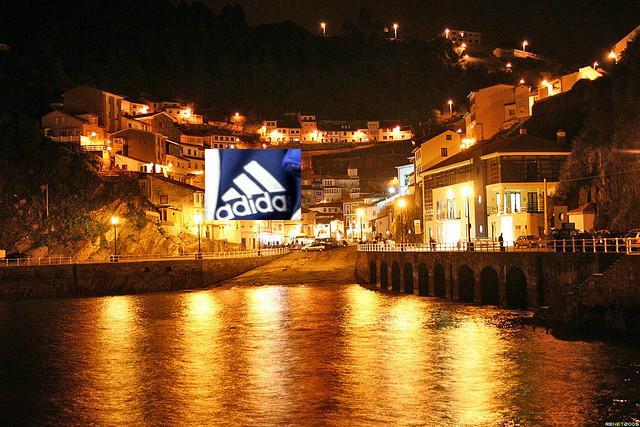
\includegraphics[width=25mm]{images/mt/flbl1.jpg} &   
\includegraphics[width=25mm]{images/mt/flbl2.jpg}  & 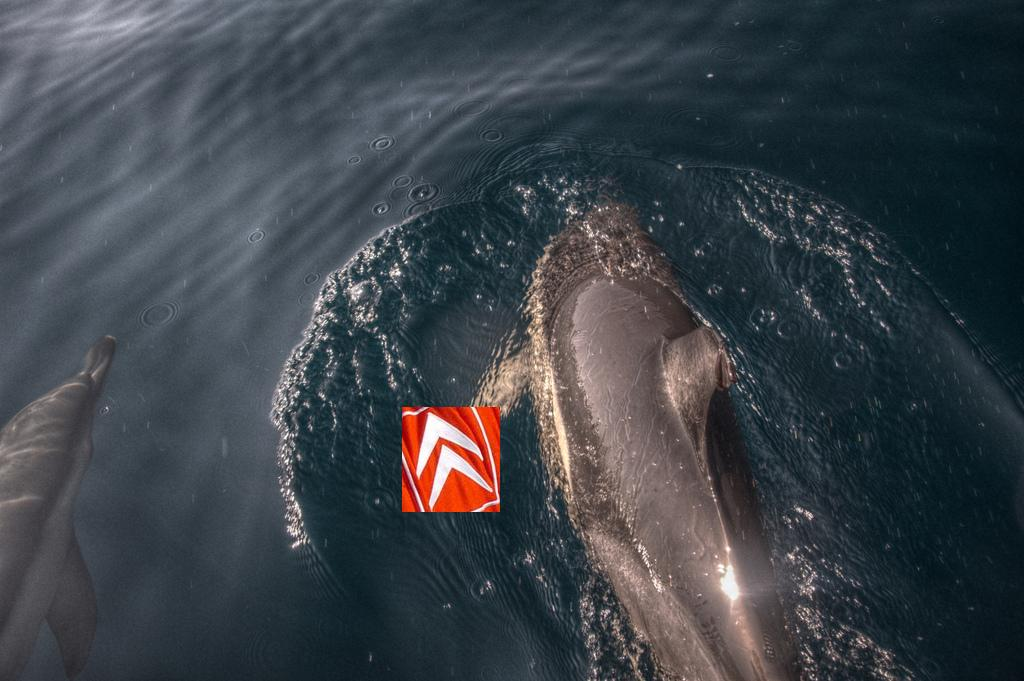
\includegraphics[width=25mm]{images/mt/flbl3.jpg} &   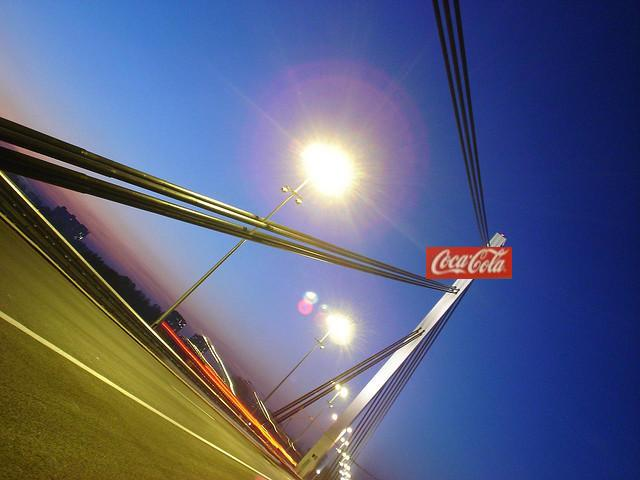
\includegraphics[width=25mm]{images/mt/flbl4.jpg} \\
    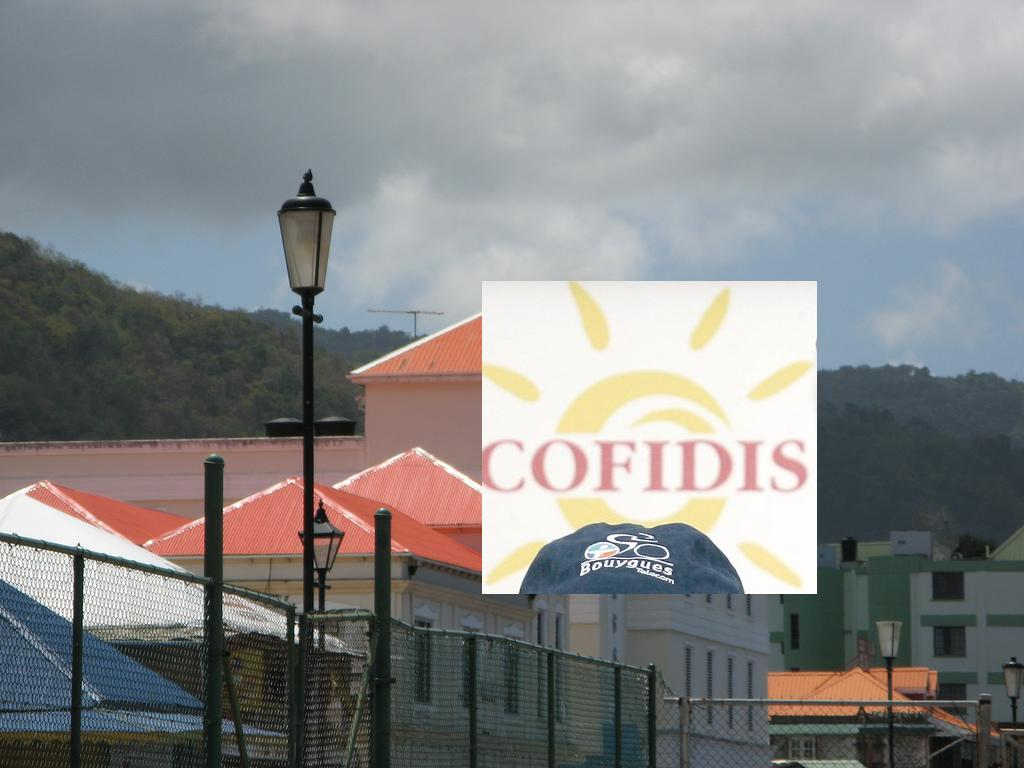
\includegraphics[width=25mm]{images/mt/flbl5.jpg} &   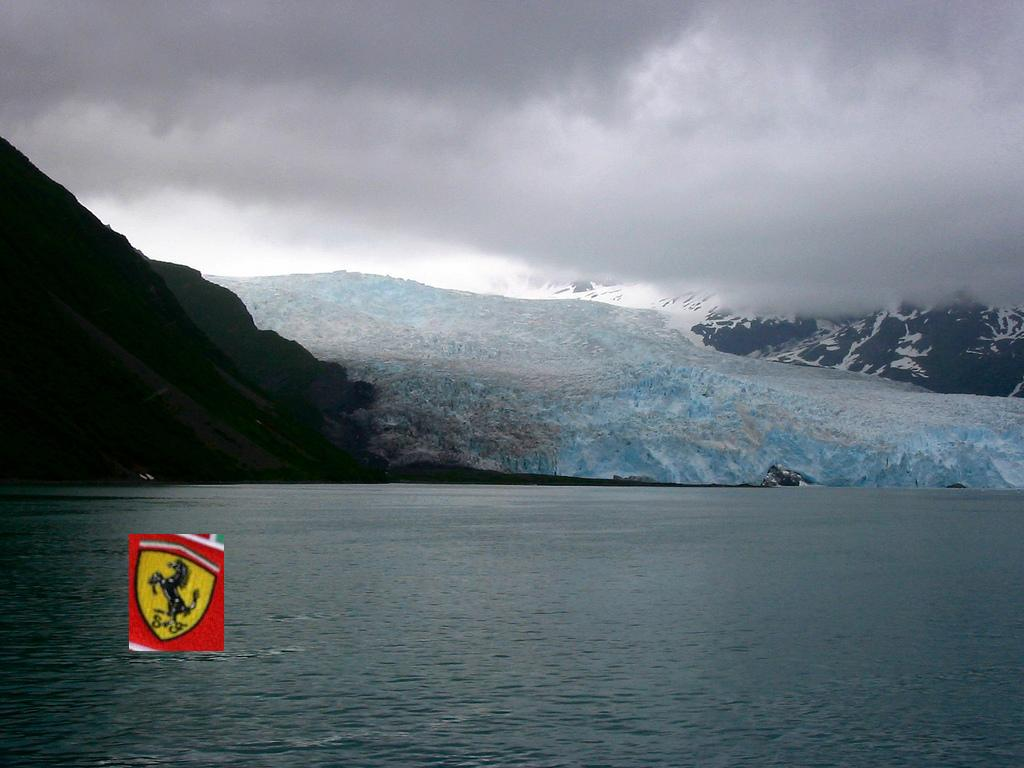
\includegraphics[width=25mm]{images/mt/flbl6.jpg}  & 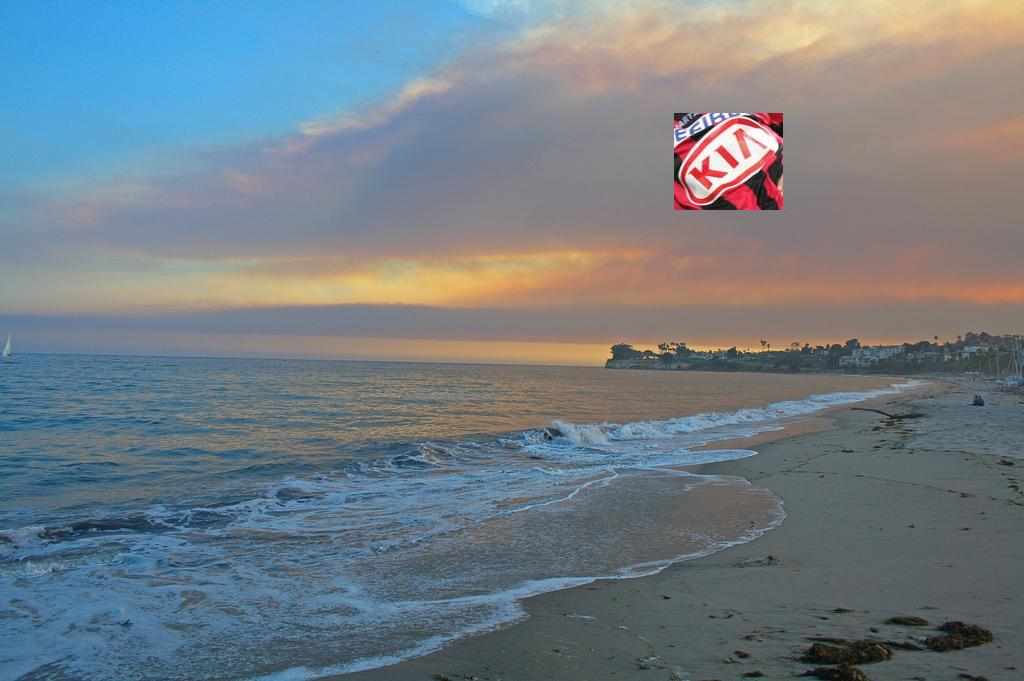
\includegraphics[width=25mm]{images/mt/flbl7.jpg} &   
\includegraphics[width=25mm]{images/mt/flbl8.jpg} 
\end{tabular}
\caption{FlickrBelgaLogos examples}
\end{figure}

This dataset was evaluated for training purposes. Therefore a small subset of BelgaLogos was chosen as test set. The logos on these images were left out from the FlickrBelgaLogos dataset. The rest of the images is used as the train set to train a Faster R-CNN model with the 37 classes of BelgaLogos. The trained models are tested on the chosen test set of BelgaLogos. Then the train set of BelgaLogos was also trained with the same network, to compare the results. After that the datasets were fused to examine the possibility of achieving better performance. Lastly, the model was trained with Curriculum Learning \cite{Bengio_curriculumlearning} (CL) as it was done with logos in \cite{DBLP:journals/corr/SuZG16}. CL is a learning process, whereas the examples became gradually more difficult during training. In this context, it is realized by training the network first merely with synthetic logos and then with real images.
\bigbreak
The synthetic dataset alone could achieve moderate results, the obvious advantage of a real dataset can be seen in figure \ref{f:flbltrain}. Unfortunately, the fusion of datasets does not yield extra performance, neither with a simple fusion, nor with Curriculum Learning. The latter has the advantage of achieving convergence much earlier, compared to other training scenarios. In \cite{DBLP:journals/corr/SuZG16}, 10\% relative extra performance was achieved by training with CL, to recognize a restricted number of classes. In case of FlickrBelgaLogos, this expected to be unsuccessful, because the same logos of BelgaLogos are reused in FlickrBelgaLogos. This means, while trying to achieve better performance, the transfer of logos to another context does not give additional information. As base network the \texttt{VGG\_CNN\_M} \cite{Chatfield14} was chosen, pretrained on ImageNet \cite{imagenet_cvpr09}, because of its much shorter training times, compared to VGG-16 (about a quarter as much time), still having a performance good enough for the experiments.
\begin{figure}
  \centering
  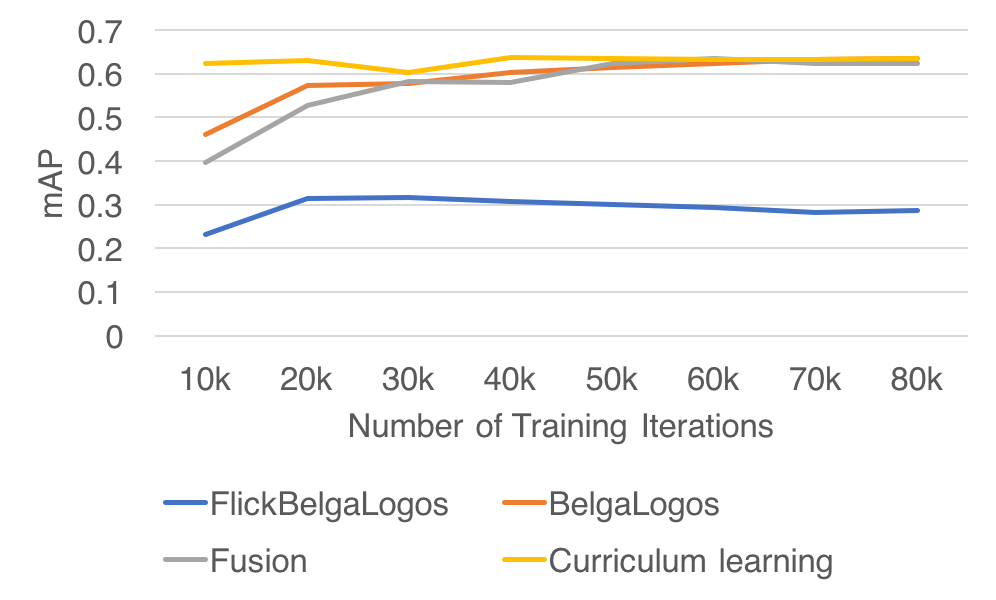
\includegraphics[width=80mm]{images/mt/bltest.png}
  \caption{Logo recognition performance after training with real (BelgaLogos) and synthetic data (FlickrBelgaLogos)}
  \label{f:flbltrain}
\end{figure}

After that, the open-set logo detection capability of the model, trained only on FlickrBelgaLogos, was tested. A Faster R-CNN was trained purely for logo detection, without logo classes. For evaluation, a self annotated dataset of a sport video was used, that has logos merely from such companies, with which the net has not been trained before. Despite the small size and the unreality of this dataset, it is able to generalize from the learned logos and detect some of the logos unknown for the network. The detection performance evaluation can be seen in figure \ref{f:flbldeteval} as well as an example detection on figure \ref{f:flbldetexample}.

\begin{figure}
  \centering
  \begin{tabular}{cc}
    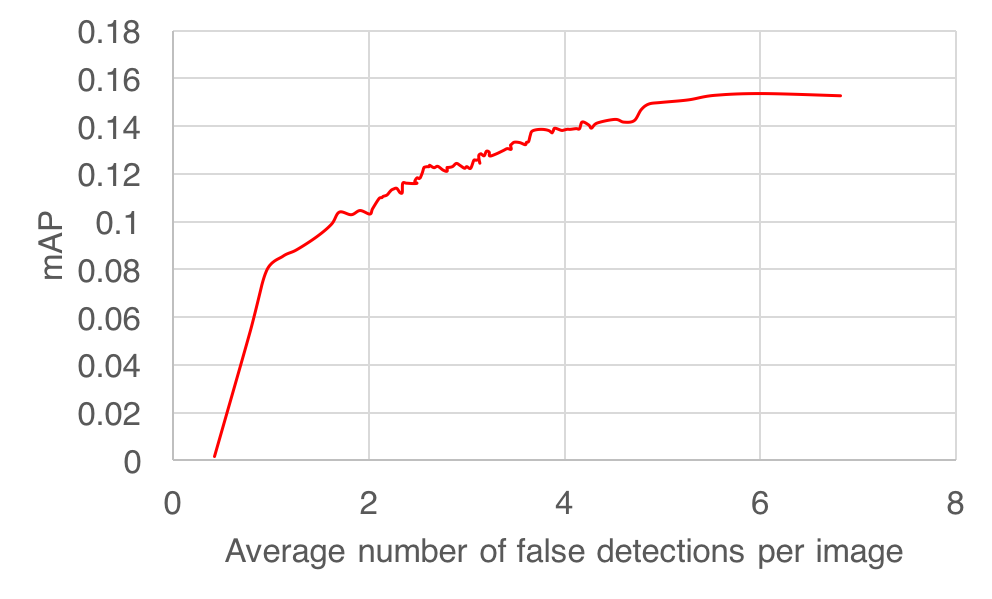
\includegraphics[width=80mm]{images/mt/flbl_det_map.png} & 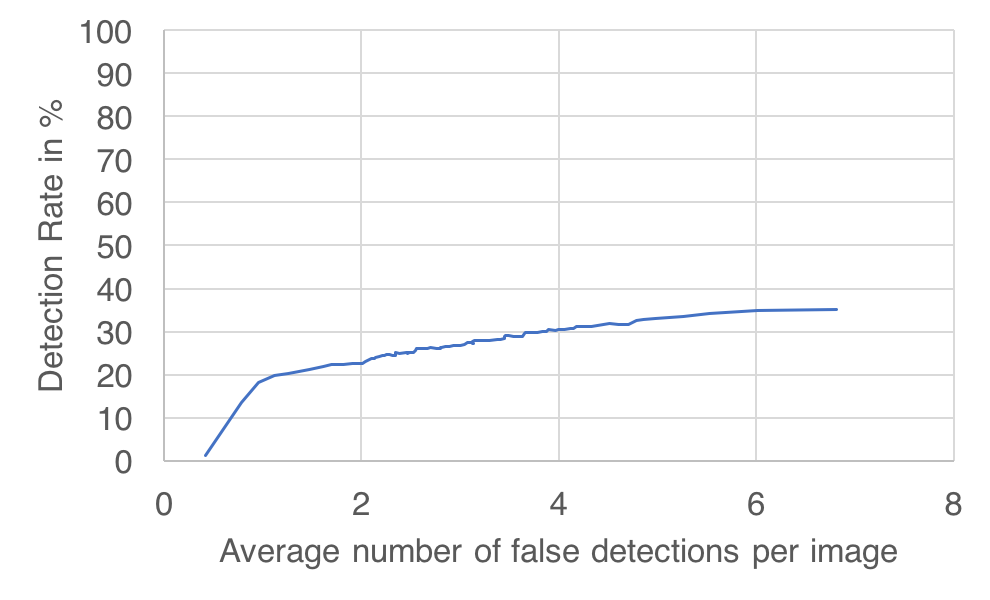
\includegraphics[width=80mm]{images/mt/flbl_det_froc.png}
  \end{tabular}
  \caption{Logo detection performance while training purely with synthetic data}
  \label{f:flbldeteval}
\end{figure}
\begin{figure}
  \centering
  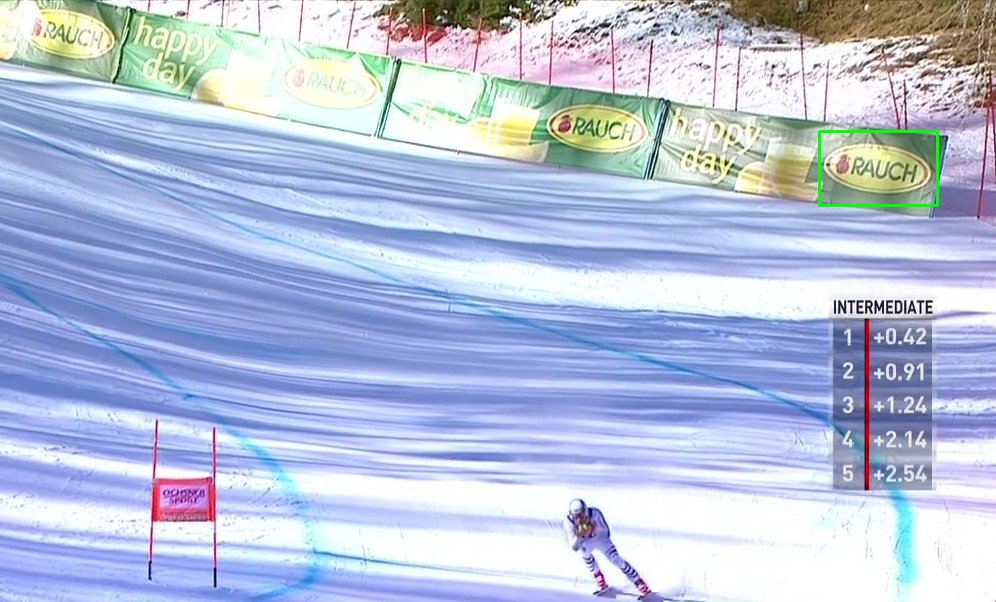
\includegraphics[width=80mm]{images/mt/flbl_det.png}
  \caption{Logo detection example by a detector, trained only with synthetic data}
  \label{f:flbldetexample}
\end{figure}
\bigbreak
\subsection{METU Trademark Dataset}\label{ss:metu}

In order to extend the training dataset, a synthetic dataset was generated, where one logo from the METU Trademark dataset \cite{DBLP:journals/corr/TursunAK17} was placed on an image. As basis, photos from Tripadvisor were used to fulfill the requirement of being practically logo-free. The majority of the logo's background has a white color. But logos usually have some background other than white. Therefore some transformations were applied on the logo images before training as follows. One third of the dataset was left unchanged. The brightness of the rest of them was adjusted to the brightness of the image, on which the logo is placed. Furthermore for one third of the logos, the mean HSV value of each logo was calculated and the hue value is rotated with 90 degree. In addition, Gaussian blur was applied on the edges of the logos, in order to suppress the sharp contrast changes. The table \ref{table:logotransformations} summarizes the applied transformations.

\begin{table}[ht!]
\centering
\begin{tabular}{|c|c|c|}
\hline \textbf{Logos} & \textbf{Hue rotation} & \textbf{Brightness adjustment} \\
\hline
\textbf{33\%} & no & no \\
\hline
\textbf{33\%} & no & yes \\
\hline
\textbf{33\%} & yes & yes \\ \hline
\end{tabular}
\caption{Applied transformations}
\label{table:logotransformations}
\end{table}

The created dataset is then used to train a two class Faster R-CNN for logo detection. The base network is again \texttt{VGG\_CNN\_M}, as in section \ref{ss:flickrbelgalogos}. For evaluation, the same self annotated sport video dataset was used, as in section \ref{ss:flickrbelgalogos}. Unfortunately, the trained network was incapable of detecting logos. The problem is most likely because of the dataset, which consists mainly of logos with a white background and a black text on them. The other source of problem could be the unreal appearance of the logos or the transformations applied to them. Figure \ref{f:synmetu} shows some generated examples.

\begin{figure}
  \centering
  \begin{tabular}{cccc}
    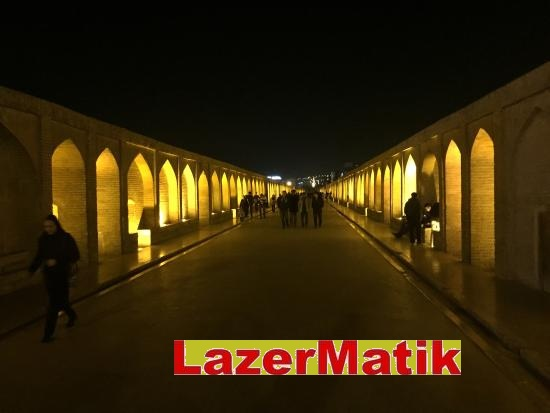
\includegraphics[height=20mm]{images/mt/synmetu1.jpg} &   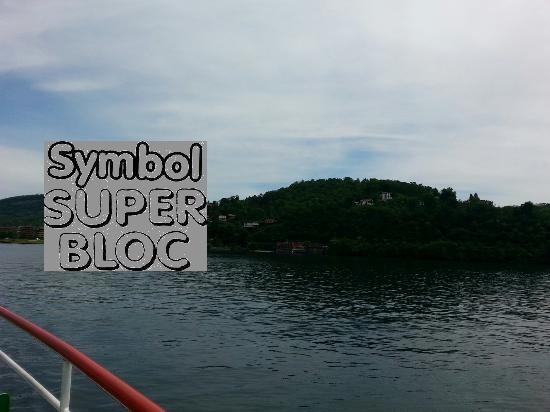
\includegraphics[height=20mm]{images/mt/synmetu2.jpg}  & 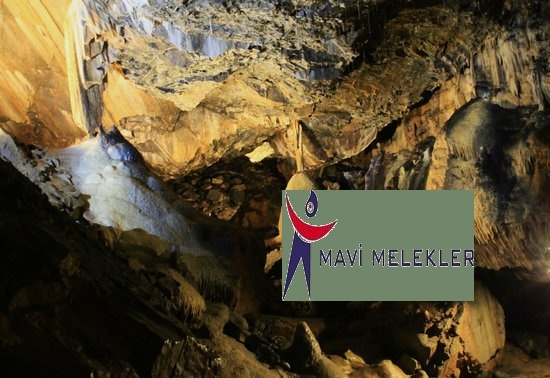
\includegraphics[height=20mm]{images/mt/synmetu3.jpg} &   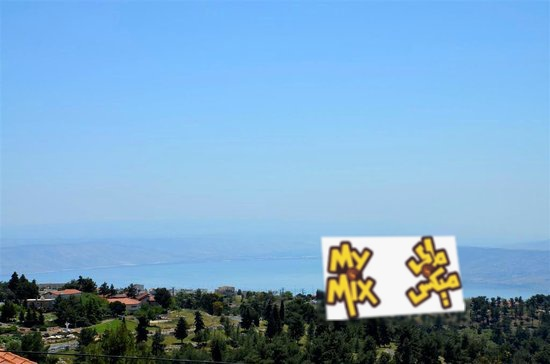
\includegraphics[height=20mm]{images/mt/synmetu4.jpg}\\
    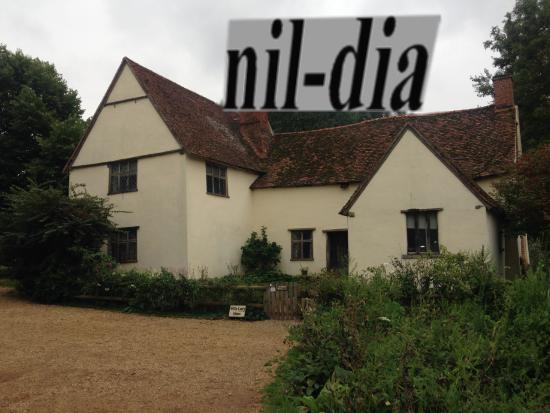
\includegraphics[height=20mm]{images/mt/synmetu5.jpg} &   
\includegraphics[height=20mm]{images/mt/synmetu6.jpg}  & 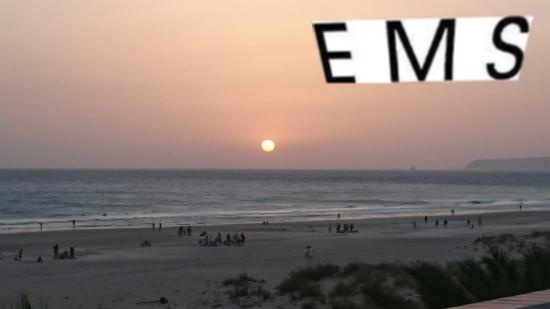
\includegraphics[height=20mm]{images/mt/synmetu7.jpg} &   
\includegraphics[height=20mm]{images/mt/synmetu8.jpg}
  \end{tabular}
  \caption{Generated synthetic logo images based on the METU Trademark Dataset \cite{DBLP:journals/corr/TursunAK17}}
  \label{f:synmetu}
\end{figure}

\subsection{Synthetic Data with Shape Based Logos}

As section \ref{ss:metu} shows, the most of the text based logos are incapable to train a model to detect real logos. In order to successfully extend the training dataset, logo images with more shape and color were collected from the Logo API of Clearbit \cite{LogoClearbit}. The logos were simply copied and pasted to the same Tripadvisor dataset, as in section \ref{ss:metu}. Unfortunately, also this dataset was not able to recognize any real logos. As a next trial, the white background of the logos was set to transparent, as suggested in \cite{DBLP:journals/corr/SuZG16}, but in the context of open-set logo detection, it does not appear to be useful either. The reason for the success of FlickrBelgaLogos, seen in section \ref{ss:flickrbelgalogos}, was most likely because the logos and their direct surroundings come from a real scene, and the logos were from the same closed-set of brands.
\bigbreak
\begin{figure}
  \centering
\begin{tabular}{cccc}
  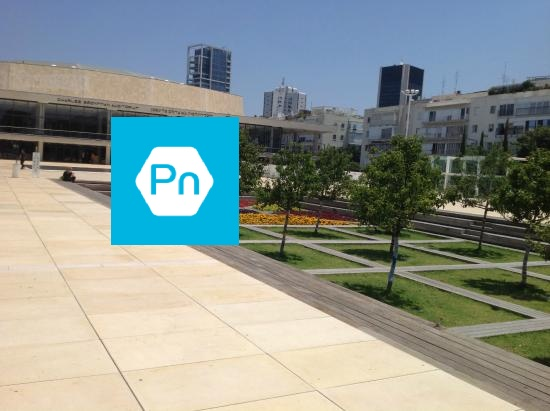
\includegraphics[height=20mm]{images/mt/clearbit1.jpg} &   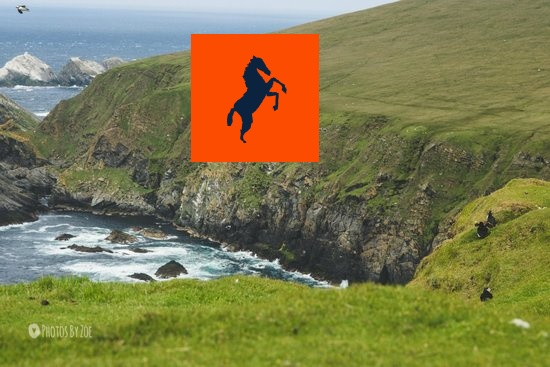
\includegraphics[height=20mm]{images/mt/clearbit2.jpg}  & 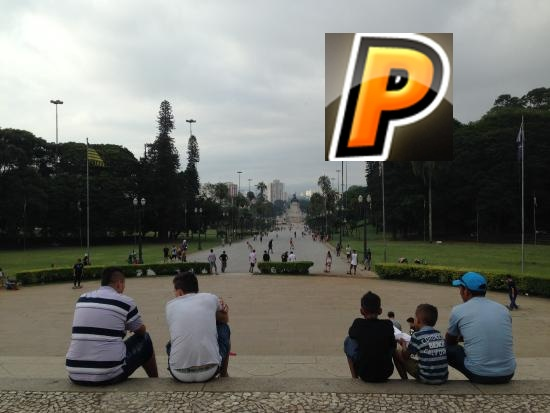
\includegraphics[height=20mm]{images/mt/clearbit3.jpg} &   
\includegraphics[height=20mm]{images/mt/clearbit4.jpg}
\end{tabular}
\caption{Generated synthetic logo images based on logo images collected from the Logo API of Clearbit \cite{LogoClearbit}}
\label{f:synlogo}
\end{figure}
\bigbreak
\section{Evaluation on FlickrLogos-32}\label{s:fleval}
The majority of logo retrieval research uses the test set of FlickrLogos-32 (FL-32) for evaluation. Therefore, the effect of additional data and different architectures to the performance was examined on this dataset. The trained networks are the following ones:
\begin{enumerate}
    \item\label{i:first} A Faster R-CNN, with \texttt{VGG\_CNN\_M\_1024} as base network, trained on the training and validation set of FL-32.
    \item\label{i:second} A jointly trained detector and classifier, as introduced in section \ref{ss:solution4}, whereas the impact of further semi-labeled data is examined by training the classifier the same way, as in point \ref{i:first}, and the detector on every other public dataset without specific brand label.
    \item\label{i:third} A faster R-CNN is trained, based on \texttt{VGG\_CNN\_M\_1024}, on the same dataset as the detector and classifier together in point \ref{i:second}, but this time with complete brand specification.
    \item Point \ref{i:first} is repeated with VGG-16.
    \item Point \ref{i:second} is repeated with VGG-16.
    \item A Faster R-CNN, trained on all public datasets, and annotated sport videos.
\end{enumerate}

The test set of FL-32 is evaluated with the configurations from points \ref{i:first}, \ref{i:second} and \ref{i:third}, and compared in figure \ref{f:vggcnnmfltest}. The networks are evaluated based on the mAP. It can be seen, that additional logo dataset, even without brand indication, can be utilized, to detect and recognize known logos with better performance by using the Siamese-like architecture, proposed in \ref{ss:solution4}. The network, trained on complete class information, begins with a worse performance due to the higher number of iterations required to distinguish in the set of learned classes with a significantly higher cardinality. Later on, it has obviously superior performance.

\begin{figure}
  \centering
  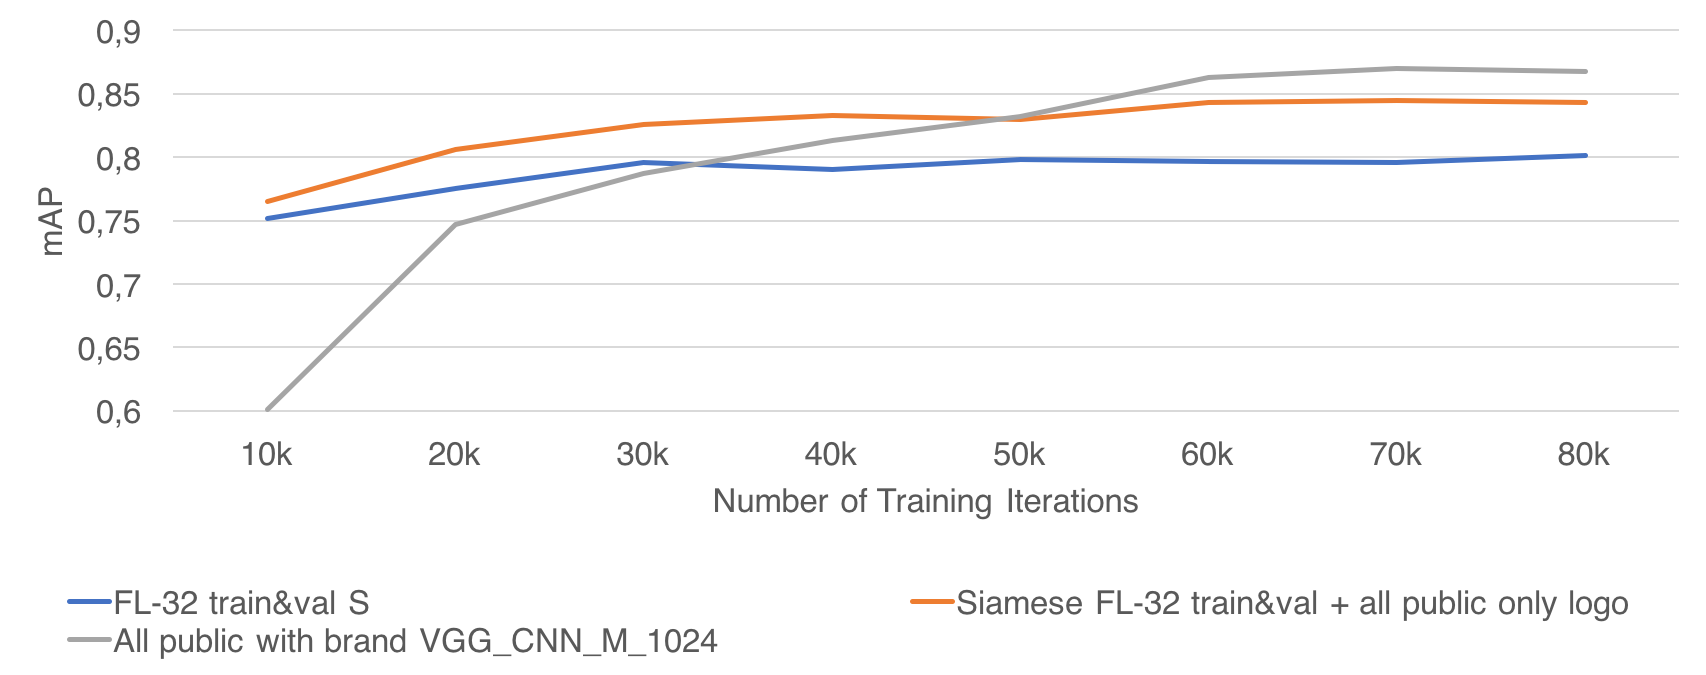
\includegraphics[width=150mm]{images/mt/vggcnnmfltest.png}
  \caption{FL-32 test evaluation with \texttt{VGG\_CNN\_M\_1024} base network}
  \label{f:vggcnnmfltest}
\end{figure}

The improvement of additional data on the performance is then tested with VGG16 base network, having more capacity. Due to more data, it achieves naturally state-of the-art performance on FL-32 test set with 90.2 mAP, whereas the best published result is 84.2 mAP, proposed by \cite{Bao:2016:RCL:3007669.3007728}. Figure \ref{f:vgg16fltest} shows the performance with VGG-16 base network, compared with the best system using \texttt{VGG\_CNN\_M\_1024}, as base network.

\begin{figure}
  \centering
  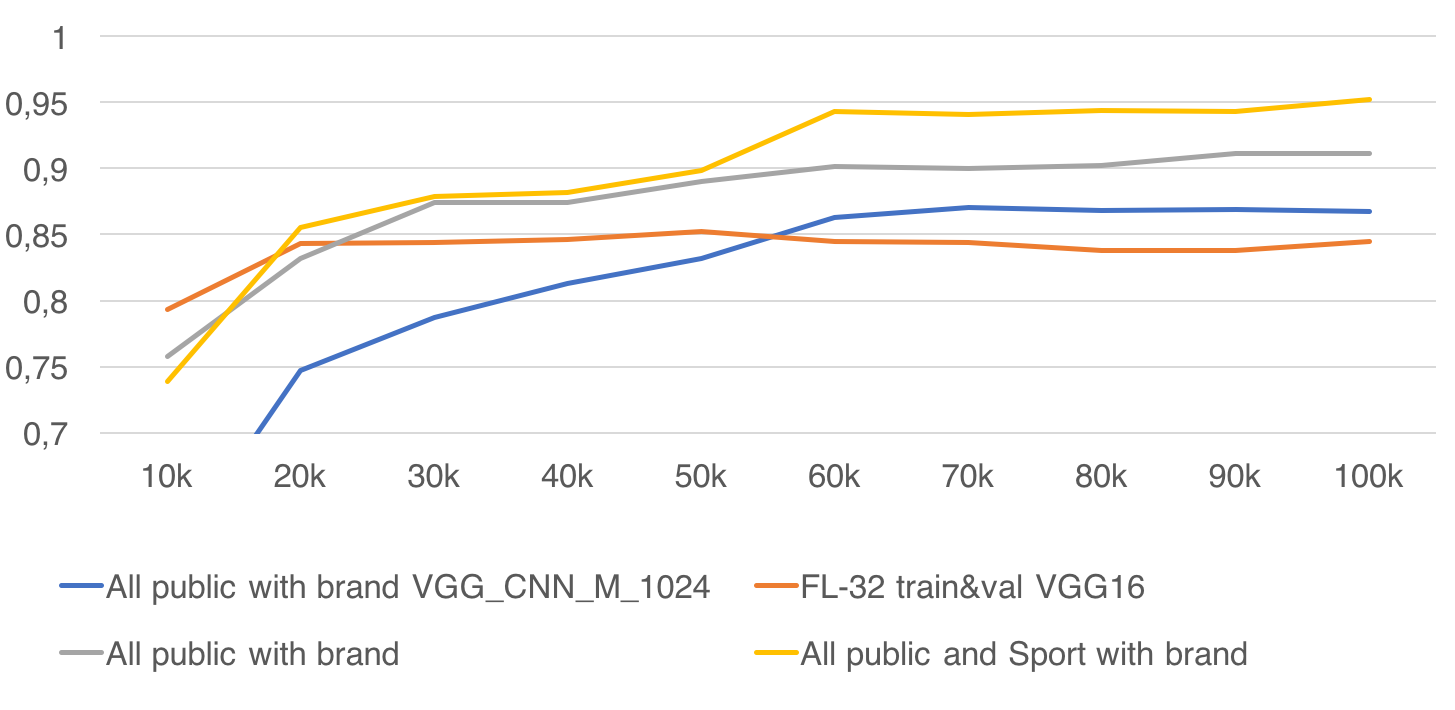
\includegraphics[width=150mm]{images/mt/vgg16fltest.png}
  \caption{FL-32 test evaluation with VGG-16 compared with the best \texttt{VGG\_CNN\_M\_1024}, as base network}
  \label{f:vgg16fltest}
\end{figure}